% =====================================================================
% THIS FILE IS THE SOURCE. Edit it, then rebuild the PDF with:
%     bash tools/compile.sh Unit_02_Probability_and_Random_Variables
% (run from the Course_Rewrite folder; it compiles twice and reports
%  page count, overfull boxes, and em dashes)
%
% Do not edit the PDF directly. Figures are the fig_*.pdf files in this
% folder, regenerated by tools/make_module*_slide_figs.py.
%
% Originally converted from the 15-module draft by a one-shot script now
% parked in tools/one_shot_generators/. Re-running those would discard
% anything you change here, so they are kept out of tools/ on purpose.
% =====================================================================
\documentclass[aspectratio=169]{beamer}
\usetheme{default}
\usefonttheme{professionalfonts}
\usepackage{amsmath, amssymb, amsfonts}
\usepackage{graphicx}
\usepackage{booktabs}
\usepackage{bm}
\usepackage{hyperref}

\mode<presentation> {
    \usetheme{Frankfurt}
    \usecolortheme{default}
}

% == notation shortcuts ==
\newcommand{\xbar}{\bar{x}}
\newcommand{\PR}[1]{P(#1)}
\newcommand{\E}[1]{E[#1]}
\newcommand{\Var}[1]{\mathrm{Var}(#1)}
\newcommand{\SD}[1]{\mathrm{SD}(#1)}

% Recurring motifs (color-coded).
\newenvironment{principle}[1]{\begin{block}{\textbf{Principle:} #1}}{\end{block}}
\newenvironment{trap}[1]{\begin{alertblock}{\textbf{Trap:} #1}}{\end{alertblock}}
\newenvironment{practice}[1]{\begin{exampleblock}{\textbf{In practice:} #1}}{\end{exampleblock}}
\newenvironment{interview}[1]{\begin{exampleblock}{\textbf{You may be asked:} #1}}{\end{exampleblock}}
\newenvironment{yourturn}[1]{%
  \setbeamercolor{block title}{fg=white,bg=orange!80!black}%
  \setbeamercolor{block body}{bg=orange!12}%
  \begin{block}{\textbf{Your turn:} #1}}{\end{block}}
\newenvironment{livedemo}[1]{%
  \setbeamercolor{block title}{fg=white,bg=teal!80!black}%
  \setbeamercolor{block body}{bg=teal!12}%
  \begin{block}{\textbf{Live demo:} #1}}{\end{block}}
\newenvironment{llmcheck}[1]{%
  \setbeamercolor{block title}{fg=white,bg=violet!75!black}%
  \setbeamercolor{block body}{bg=violet!10}%
  \begin{block}{\textbf{LLM check:} #1}}{\end{block}}

\title{Probability and Random Variables}
\subtitle{Unit 2: What Chance Produces, and How to Put a Number on It}
\author{Stat 220 \textbar{} Statistics for Data Science}
\date{}

\begin{document}

\begin{frame}
  \titlepage
\end{frame}

% ======================================================================
\section{Randomness}
% ======================================================================
\begin{frame}{The thing we assumed last unit}
\begin{itemize}
  \item Unit 1 kept asking: \emph{what would this look like if nothing were going on?} We answered
        it by hand for the Coke test and then waved at it everywhere else.
  \item To answer it in general, we need the machinery: how to describe a random process, combine
        events, and attach a number to an uncertain outcome.
  \item That is this unit. Three days: what randomness looks like, how evidence updates it, and
        how to summarize an uncertain quantity with a mean and a spread.
\end{itemize}
\begin{principle}{probability is a claim about a process, not about one outcome}
``There is a 30\% chance of rain'' is a statement about how often days like this one end in rain.
No single afternoon can prove it right or wrong.
\end{principle}
\end{frame}

\begin{frame}{Live experiment: can you fake a coin?}
\begin{livedemo}{everyone is on the fool-me team}
No honest flippers this time. \textbf{All of you} invent a sequence of \textbf{50} H's and T's
that looks random enough to pass for a real coin.
\begin{itemize}
  \item Write it out by hand. No coins, no random number generators, no phones.
  \item Then type it into the detector and it will tell you, in front of everyone, whether a
        person wrote it.
\end{itemize}
\end{livedemo}
\vspace{0.2em}
{\tiny\textit{Materials: paper, and \texttt{tools/coin\_detector.py} projected. Time: 6 minutes to
write, 8 to run people through it.}}
\centering\small
I flipped a real coin 50 times, 120 times over, before class. Your sequence gets compared against
those.
\end{frame}

\begin{frame}{Stay here while they write: what gives you away}
The detector does not count heads. Both real and invented sequences land near 25. It looks at two
things:
\begin{itemize}
  \item \textbf{Your longest run} of the same side in a row. Across my 120 real sequences the
        longest run averaged \textbf{5.8}, and only \textbf{22\%} had a longest run of 4 or
        shorter. Invented sequences almost never go past 4, because a run of six does not
        \emph{feel} random.
  \item \textbf{How often you switch sides.} Real coins alternate about \textbf{50\%} of the time.
        People alternate 60 to 75\% of the time, because switching feels like what randomness
        should do.
\end{itemize}
\begin{practice}{the judgment this is really about}
``Here is a pattern in our data. Is it real, or is it what randomness looks like?'' You will make
this call more often than any other judgment in applied work.
\end{practice}
\end{frame}

\begin{frame}{The reveal: look at the streaks}
\begin{columns}[c]
\begin{column}{0.58\textwidth}
\centering
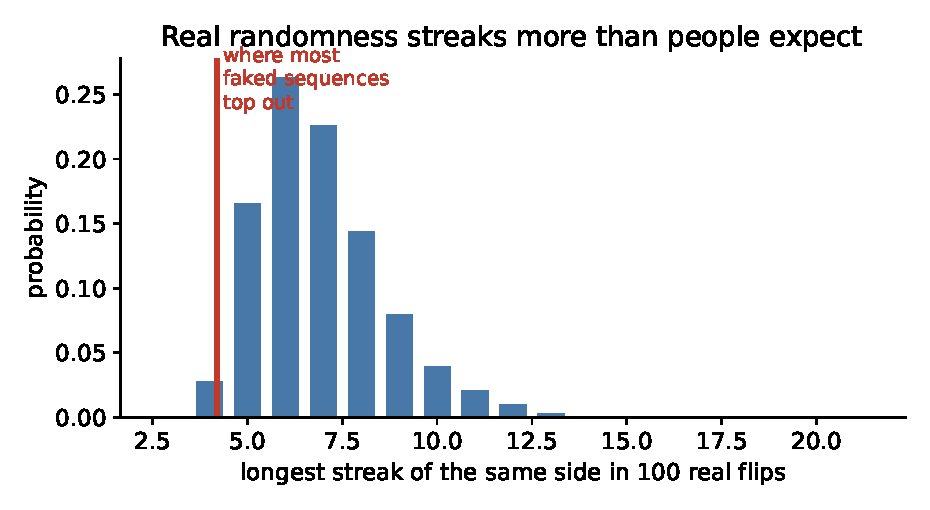
\includegraphics[width=\textwidth]{fig_m05_streaks.pdf}
\end{column}
\begin{column}{0.42\textwidth}
\small
In my 120 pre-flipped sequences the longest streak averaged \textbf{5.8}, and ran as high as
\textbf{12}.
\begin{itemize}
  \item Invented sequences top out around 4.
  \item Real randomness \textbf{clumps}. Invented sequences spread out too evenly, and that is what
        gives them away.
\end{itemize}
\end{column}
\end{columns}
\onslide<2->{\centering\small
Count how many I got right. This is not a superpower: I know the distribution of a streak length,
and you were guessing.}
\end{frame}

\begin{frame}{Why that game matters at work}
\begin{itemize}
  \item Three support tickets in one week from the same region. A pattern, or a clump?
  \item Four straight bad quarters for one sales rep. A slump, or a streak?
  \item A cluster of server failures on Tuesdays. A cause, or a coincidence?
\end{itemize}
\begin{principle}{the null hypothesis of everyday life}
Before you explain a pattern, work out what pure chance would have produced. Most ``patterns'' in
small data are exactly the clumping you failed to imagine.
\end{principle}
\end{frame}

\begin{frame}{What this unit gives you}
\begin{columns}[T]
\begin{column}{0.5\textwidth}
\textbf{Things to know}
\begin{itemize}\small
  \item the rules for combining events, and what independence really requires
  \item conditional probability, and why $\PR{A \mid B} \ne \PR{B \mid A}$
  \item Bayes' rule, and the decisive role of the base rate
  \item expectation and variance, and what happens when you add things up
  \item which standard distribution matches which real-world story
\end{itemize}
\end{column}
\begin{column}{0.5\textwidth}
\textbf{Mistakes to stop making}
\begin{itemize}\small
  \item flipping a conditional probability around
  \item ignoring the base rate after a positive test
  \item multiplying probabilities that were never independent
  \item expecting chance to ``even out'' in the short run
  \item reporting a mean with no spread, or calling it typical when the data is skewed
  \item plugging averages into a nonlinear calculation
\end{itemize}
\end{column}
\end{columns}
\end{frame}

\begin{frame}{The vocabulary, quickly}
\begin{itemize}
  \item An \textbf{experiment} is any process with an uncertain outcome: a flip, a customer visit,
        a quarter of sales.
  \item The \textbf{sample space} is everything that could happen.
  \item An \textbf{event} is a subset of that: ``the customer buys,'' ``revenue tops \$1M.''
  \item $\PR{A}$ is a number in $[0,1]$ measuring how often $A$ happens if the process runs many
        times.
\end{itemize}
\begin{principle}{name the sample space first}
Most probability errors are not arithmetic errors. They are errors about \emph{which set of
outcomes we are talking about}.
\end{principle}
\end{frame}

\begin{frame}{Three rules that generate everything else}
\begin{enumerate}
  \item \textbf{Complement:} $\PR{\text{not } A} = 1 - \PR{A}$.
  \item \textbf{Addition:} $\PR{A \text{ or } B} = \PR{A} + \PR{B} - \PR{A \text{ and } B}$.
        Subtract the overlap so it is not counted twice.
  \item \textbf{Multiplication:} $\PR{A \text{ and } B} = \PR{A}\,\PR{B \mid A}$.
        \emph{Always} true. That $\PR{B \mid A}$ is a \textbf{conditional} probability, defined
        on the next slide, and it collapses to $\PR{A}\PR{B}$ only when the two are independent.
\end{enumerate}
\begin{trap}{the shortcut everyone takes}
Multiplying $\PR{A}\PR{B}$ is the most common probability error in industry, because independence
gets assumed silently instead of argued for.
\end{trap}
\end{frame}

\begin{frame}{The complement rule is your best friend}
``At least one'' problems are almost always easier backwards:
\[
\PR{\text{at least one failure}} = 1 - \PR{\text{no failures}}.
\]
\begin{itemize}
  \item A service fails on a given day with probability 0.01. Over a 90-day quarter, if days were
        independent,
        $\PR{\text{at least one outage}} = 1 - 0.99^{90} \approx \mathbf{0.60}$.
  \item A 1\% daily risk is a coin flip over a quarter. Rare events stop being rare once you get
        many chances at them.
\end{itemize}
\begin{principle}{count the chances, not the impressions}
``That basically never happens'' is a statement about one trial. Always ask how many trials there
are.
\end{principle}
\end{frame}

\begin{frame}{Conditional probability: shrinking the world}
\[
\PR{A \mid B} = \frac{\PR{A \text{ and } B}}{\PR{B}}
\]
\begin{itemize}
  \item Read it as: \emph{throw away every outcome where $B$ did not happen}, then ask how often
        $A$ happens among what is left.
  \item Conditioning is what data science actually does. Every model output is a conditional
        statement: given these features, what do we expect?
\end{itemize}
\begin{principle}{a probability without a condition is incomplete}
``What is the churn rate?'' is a worse question than ``what is the churn rate \emph{for accounts
under \$500 a month in their first year}?''
\end{principle}
\end{frame}

\begin{frame}{Independence, stated carefully}
$A$ and $B$ are \textbf{independent} when knowing one tells you nothing about the other:
\[
\PR{A \mid B} = \PR{A}.
\]
\begin{itemize}
  \item Two coin flips: independent.
  \item Two mortgages in the same city defaulting: \alert{not} independent. They share a housing
        market.
  \item Two servers in the same rack failing: not independent. They share power, cooling, and a
        deploy pipeline.
\end{itemize}
\begin{principle}{ask what they share}
Things are dependent when they share a cause. Go looking for the shared cause before you assume
independence.
\end{principle}
\end{frame}

\begin{frame}{Why false independence is expensive}
\begin{itemize}
  \item In 2008, models priced pools of mortgages by treating individual defaults as nearly
        independent. Under that assumption, the chance that a huge fraction defaulted at once was
        effectively zero.
  \item Defaults were driven by a common factor, the national housing market. When it turned, they
        turned together.
  \item The model was not wrong about any single mortgage. It was wrong about the
        \textbf{dependence}, and that was enough to matter.
\end{itemize}
\begin{trap}{independence is an assumption, not a fact}
Multiplying small probabilities makes catastrophes look impossible. That is exactly when to
double-check whether the events share a driver.
\end{trap}
\end{frame}

\begin{frame}{Your turn \#1}
\begin{yourturn}{is the multiplication legitimate?}
An engineer says: ``Each of our three data centers has a 1\% chance of going down in a given
month, so the chance all three are down at once is $0.01^3 = $ one in a million. We are fine.''
\vspace{0.3em}

Turn to a neighbor: what would have to be true for that number to be right, and would you bet the
company on it?
\end{yourturn}
\end{frame}

\begin{frame}{Your turn \#1: answer}
\begin{itemize}
  \item The calculation requires the three outages to be \textbf{independent}.
  \item They are not. A bad deploy, an expired certificate, a cloud-provider outage, a BGP
        misconfiguration, or an attack hits all three at once.
  \item The honest statement: one in a million is a \emph{lower bound under the most optimistic
        possible assumption}, and the real risk is dominated by the shared causes.
\end{itemize}
\begin{principle}{correlated failures are the ones that kill you}
When you build redundancy you are betting on independence. Spend your effort making the failures
independent, not on adding a fourth copy of the same thing behind the same load balancer.
\end{principle}
\end{frame}

\begin{frame}{Two more things randomness does that surprise people}
\begin{columns}[c]
\begin{column}{0.5\textwidth}
\centering
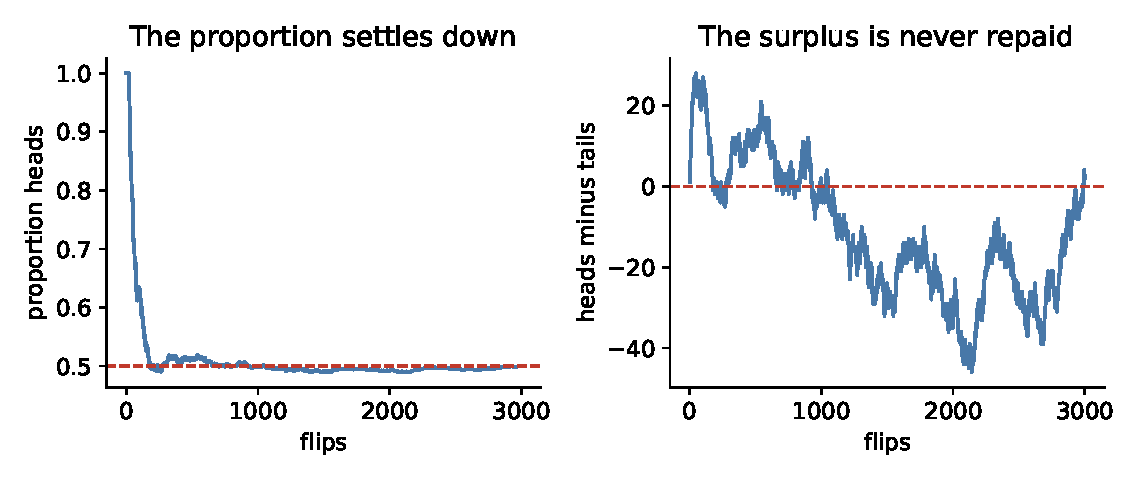
\includegraphics[width=\textwidth]{fig_m05_lln.pdf}
\end{column}
\begin{column}{0.5\textwidth}
\small
\textbf{The coin is never ``due.''} After a run of heads, the \emph{proportion} drifts back toward
one half because later flips swamp the early surplus. The surplus itself is never repaid, only
diluted.
\vspace{0.5em}

\textbf{Small groups produce the extremes.} The counties with the lowest cancer rates are mostly
small rural ones. So are the counties with the highest. Same cause: tiny denominators.
\end{column}
\end{columns}
\end{frame}

\begin{frame}{Coincidences are more common than they feel}
\begin{columns}[c]
\begin{column}{0.5\textwidth}
\centering
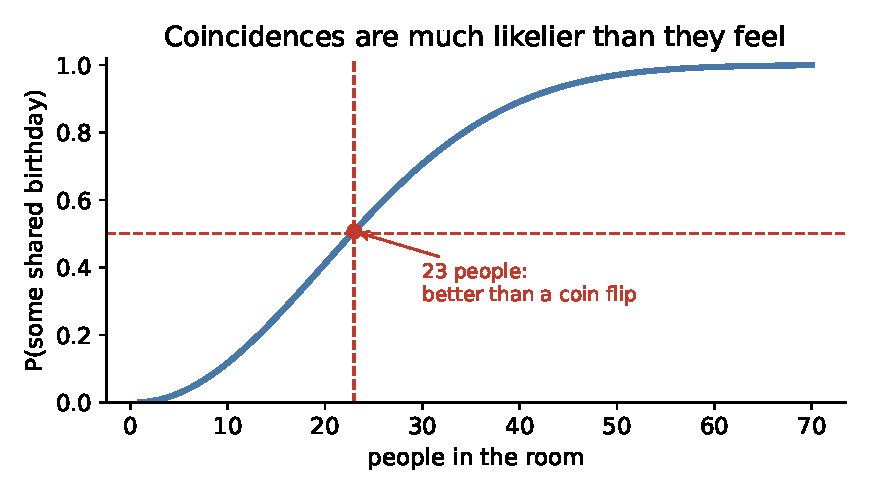
\includegraphics[width=\textwidth]{fig_m05_birthday.pdf}
\end{column}
\begin{column}{0.5\textwidth}
\small
With 23 people a shared birthday is more likely than not. With 50 it is nearly certain.
\begin{itemize}
  \item We intuit ``someone shares \emph{my} birthday,'' which is rare.
  \item The actual question involves all $\binom{23}{2} = 253$ \emph{pairs}.
\end{itemize}
Same logic on your data: test 100 variables at the 0.05 level and about five look
``significant'' by construction.
\end{column}
\end{columns}
\onslide<2->{\centering\small Let us check: does anyone here share a birthday? Months first, then
days.}
\end{frame}

% ======================================================================
\section{Conditioning}
% ======================================================================

\begin{frame}{The direction matters enormously}
$\PR{A \mid B}$ and $\PR{B \mid A}$ are different numbers, often wildly different.
\begin{itemize}
  \item $\PR{\text{speaks Spanish} \mid \text{lives in Spain}}$ is near 1.
  \item $\PR{\text{lives in Spain} \mid \text{speaks Spanish}}$ is small: most Spanish speakers
        live elsewhere.
  \item $\PR{\text{rich} \mid \text{owns a private jet}}$ is near 1. The reverse,
        $\PR{\text{owns a private jet} \mid \text{rich}}$, is not.
\end{itemize}
\begin{trap}{the prosecutor's fallacy}
``The chance of this DNA match if he were innocent is 1 in a million, so there is a 1 in a million
chance he is innocent.'' Those are different conditionals, and the second also depends on how many
people could have been the source.
\end{trap}
\end{frame}

\begin{frame}{A wrongful conviction built on a flipped conditional}
\textbf{Setup.} Sally Clark was convicted in the UK in 1999 after two of her infants died
suddenly. An expert testified that the chance of two cot deaths in one family was ``1 in 73
million,'' computed by squaring a single-death rate.
\begin{itemize}
  \item \textbf{Error 1:} the two deaths were treated as independent, ignoring shared genetics and
        environment.
  \item \textbf{Error 2:} even taken at face value, that number is
        $\PR{\text{evidence} \mid \text{innocent}}$, not
        $\PR{\text{innocent} \mid \text{evidence}}$. The alternative, a mother murdering two
        infants, is \emph{also} extremely rare, and the comparison is what matters.
\end{itemize}
The conviction was overturned in 2003, and the Royal Statistical Society issued a public statement
about the misuse of the statistic.
\end{frame}

\begin{frame}{Your turn \#2}
\begin{yourturn}{translate the claim}
A security vendor advertises: ``Our system flags fraud with 95\% accuracy.''
\vspace{0.3em}

With a neighbor, write down: (i) which conditional probability is 95\% here, (ii) which conditional
probability the fraud investigator actually cares about, and (iii) what extra number you need to
get from one to the other.
\end{yourturn}
\end{frame}

\begin{frame}{Your turn \#2: answer}
\begin{itemize}
  \item (i) The vendor means roughly $\PR{\text{flagged} \mid \text{fraud}}$, a detection rate.
  \item (ii) The investigator, holding a flagged case, needs
        $\PR{\text{fraud} \mid \text{flagged}}$. That is what decides whether the review queue is
        worth staffing.
  \item (iii) You need the \textbf{base rate} of fraud, plus the false-positive rate on the honest
        majority.
\end{itemize}
\begin{principle}{the missing number is almost always the base rate}
Accuracy claims describe the test. Decisions need the rate of the thing being tested for.
\end{principle}
\end{frame}

\begin{frame}{Bayes' rule}
\[
\PR{A \mid B} \;=\; \frac{\PR{B \mid A}\,\PR{A}}{\PR{B}}
\]
\begin{itemize}
  \item It is the formula for \textbf{reversing} a conditional, which is the operation we need
        constantly.
  \item $\PR{A}$ is the \textbf{prior}, what you believed beforehand. $\PR{A \mid B}$ is the
        \textbf{posterior}, what you believe after seeing the evidence.
  \item Unit 10 turns this into a whole way of doing inference. Today it is a tool for getting the
        direction right.
\end{itemize}
\begin{principle}{evidence updates a starting point, it does not replace one}
A positive test moves your belief. Where it moves \emph{to} depends on where it started.
\end{principle}
\end{frame}

\begin{frame}{The four numbers a test comes with}
Any yes/no test has two error rates, and they have names you will meet constantly.
\begin{center}\footnotesize
\begin{tabular}{p{0.26\textwidth} p{0.30\textwidth} p{0.32\textwidth}}
\toprule
\textbf{Name} & \textbf{Conditional probability} & \textbf{In words} \\
\midrule
Sensitivity & $\PR{\text{test}^+ \mid \text{sick}}$ & of those who have it, the share the
test catches \\
Specificity & $\PR{\text{test}^- \mid \text{healthy}}$ & of those who do not, the share it
clears \\
Prevalence & $\PR{\text{sick}}$ & how common it is to begin with \\
Predictive value & $\PR{\text{sick} \mid \text{test}^+}$ & \textbf{what the patient wants to
know} \\
\bottomrule
\end{tabular}
\end{center}
\vspace{0.3em}
\begin{principle}{the first three are given, the fourth is the answer}
Sensitivity and specificity describe the test itself. The predictive value changes with the
prevalence, which is why one test means different things in different populations.
\end{principle}
\end{frame}

\begin{frame}{Do not use the formula. Use 10,000 people.}
A disease affects \textbf{1\%} of people (the prevalence). The test catches \textbf{99\%} of
sick people (sensitivity 0.99) and is wrong on \textbf{5\%} of healthy people (specificity 0.95).
You test positive. What is the chance you are sick?
\vspace{0.4em}

Picture 10,000 people:
\begin{itemize}
  \item 100 are sick. Of those, \textbf{99} test positive.
  \item 9,900 are healthy. Of those, \textbf{495} test positive anyway.
  \item So 594 people test positive, and only 99 of them are sick.
\end{itemize}
\[
\PR{\text{sick} \mid \text{positive}} = \frac{99}{99 + 495} \approx \textbf{17\%}.
\]
\end{frame}

\begin{frame}{The same fact, as a picture}
\begin{columns}[c]
\begin{column}{0.62\textwidth}
\centering
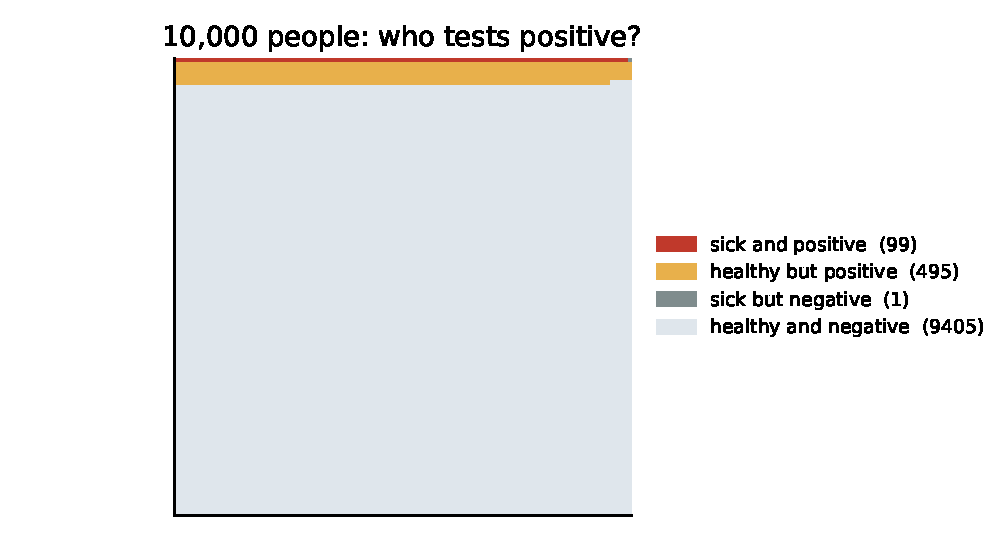
\includegraphics[width=\textwidth]{fig_m05_screening.pdf}
\end{column}
\begin{column}{0.38\textwidth}
\small
The healthy group is so much larger that its 5\% error rate produces \textbf{five times} as many
positives as the disease itself.
\vspace{0.4em}

A ``99\% accurate'' test for a rare condition is mostly a false-positive machine. No amount of
rhetoric changes the arithmetic.
\end{column}
\end{columns}
\end{frame}

\begin{frame}{Why counting people beats the formula}
\begin{itemize}
  \item Natural frequencies (99 out of 594) are far easier for humans, including doctors and
        executives, than conditional probabilities.
  \item In studies, physicians given percentages get this problem wrong most of the time. Given
        counts of patients, most get it right.
  \item Drawing the 10,000-person table is a better answer than reciting Bayes' rule, because it
        also \emph{explains} the result to whoever asked.
\end{itemize}
\begin{principle}{the move to reach for}
Whenever someone hands you a sensitivity, a specificity, and a rare condition, immediately build a
table of a big round number of people.
\end{principle}
\end{frame}

\begin{frame}{This is the churn model, the fraud flag, the spam filter}
\begin{itemize}
  \item Your model flags 500 accounts as ``about to churn.'' If churn is 2\% and your
        false-positive rate is 5\%, most of that list is not churning.
  \item That is not a broken model. It is what a rare outcome does to \emph{any} imperfect
        classifier.
  \item The fix is often not a better model but a better \textbf{base rate}: run the classifier
        only on a segment where the outcome is common.
\end{itemize}
\begin{interview}{a standard screening question}
``Your model is 99\% accurate at predicting a 1-in-1000 event. Are you impressed?'' No: predicting
``never'' scores 99.9\%. Unit 8 builds the full vocabulary for this.
\end{interview}
\end{frame}

\begin{frame}{Your turn \#3}
\begin{yourturn}{run the numbers yourself}
A drug test is 98\% accurate in both directions: it catches 98\% of users and clears 98\% of
non-users. In a workplace where \textbf{0.5\%} of employees actually use the drug, an employee
tests positive.
\vspace{0.3em}

Take 10,000 employees. How many test positive? What fraction of them are real users?
\end{yourturn}
\end{frame}

\begin{frame}{Your turn \#3: answer}
Out of 10,000 employees:
\begin{itemize}
  \item 50 are users, and 98\% of them, about \textbf{49}, test positive.
  \item 9,950 are not, and 2\% of them, \textbf{199}, test positive anyway.
  \item Positives: $49 + 199 = 248$, of whom 49 are real users. About \textbf{20\%}.
\end{itemize}
\begin{trap}{a defensible test, an indefensible decision}
Firing everyone who tests positive means firing four innocent people for every real user. The test
is fine. Using it alone as a decision rule is not.
\end{trap}
\end{frame}

% ======================================================================
\section{Random variables}
% ======================================================================
\begin{frame}{Live experiment: what will you pay to play?}
\begin{livedemo}{a sealed-bid auction for three gambles}
On a slip of paper write the \textbf{most you would pay} to play each game. One number each, no
conferring.
\begin{enumerate}
  \item \textbf{Game A:} I roll a die. You win \$60 if it shows a 6, otherwise nothing.
  \item \textbf{Game B:} I flip a coin. Heads you win \$20, tails nothing.
  \item \textbf{Game C:} I flip a coin. Heads you win \$2{,}000, tails you \emph{lose} \$1{,}000.
\end{enumerate}
\end{livedemo}
\vspace{0.2em}
{\tiny\textit{Materials: slips of paper. Time: 8 minutes. Do not reveal the expected values until the bids are collected.}}
\centering\small Pass them forward. We will find the highest bidder for each and compare the bids
to what the games are worth.
\end{frame}

\begin{frame}{Stay here while they bid: what each game is worth}
\begin{itemize}
  \item Game A: $\tfrac{1}{6}(60) + \tfrac{5}{6}(0) = \$10$.
  \item Game B: $\tfrac{1}{2}(20) + \tfrac{1}{2}(0) = \$10$.
  \item Game C: $\tfrac{1}{2}(2000) + \tfrac{1}{2}(-1000) = \$500$.
\end{itemize}
\onslide<2->{
Two predictions about your slips:
\begin{itemize}
  \item A and B are worth the same, but B usually draws higher bids. The \emph{spread} bothers
        you, not just the average.
  \item Almost nobody bids near \$500 for C, even though it is worth fifty times the others.
\end{itemize}
That instinct is correct, and it is why this day covers \textbf{two} numbers, not one.}
\end{frame}

\begin{frame}{Random variables and expectation}
A \textbf{random variable} is not ``the number that came up.'' It is the whole recipe: which
numbers are possible and how often each occurs.
\[
\E{X} \;=\; \sum_x x \cdot \PR{X = x}
\]
\begin{itemize}
  \item The expectation is the average you would see over a very large number of repetitions.
  \item It need not be a possible value: the expected number of children per family is 2.3, and no
        family has 2.3 children.
\end{itemize}
\begin{principle}{expectation answers ``in the long run,'' not ``this time''}
It is the right tool for decisions you make repeatedly, and a dangerous one for a decision you
make once with everything on the line.
\end{principle}
\end{frame}

\begin{frame}{Linearity: the most useful fact in this course}
For \emph{any} random variables, independent or not:
\[
\E{aX + b} = a\E{X} + b, \qquad \E{X + Y} = \E{X} + \E{Y}.
\]
\begin{itemize}
  \item No independence required. That is why expectations are so pleasant to work with.
  \item \textbf{Worked example.} A call center takes 400 calls a day. Each caller buys with
        probability 0.06, spending \$85. Write $R = \sum_{i=1}^{400} 85\, I_i$ where $I_i$ is 1 if
        caller $i$ buys. Then $\E{R} = 400 \times 85 \times 0.06 = \$2{,}040$.
  \item We never needed the distribution of daily revenue. Linearity gave us the mean without
        it.
\end{itemize}
\end{frame}

\begin{frame}{Variance: how far things swing}
\[
\Var{X} = \E{(X - \E{X})^2}, \qquad \SD{X} = \sqrt{\Var{X}}.
\]
\begin{itemize}
  \item Variance is in squared units (dollars squared), which nobody can interpret. Report the
        \textbf{standard deviation}, which is in the original units.
  \item $\Var{aX + b} = a^2 \Var{X}$: shifting does nothing, scaling squares.
  \item For \textbf{independent} $X$ and $Y$: $\Var{X + Y} = \Var{X} + \Var{Y}$. Variances add, so
        standard deviations grow like $\sqrt{n}$, not $n$.
\end{itemize}
\begin{trap}{the independence clause, again}
``Variances add'' is not a law of nature. It is a reward for independence, and it is the same
assumption that failed in 2008.
\end{trap}
\end{frame}

\begin{frame}{Why averaging works, and when it stops}
\begin{columns}[c]
\begin{column}{0.58\textwidth}
\centering
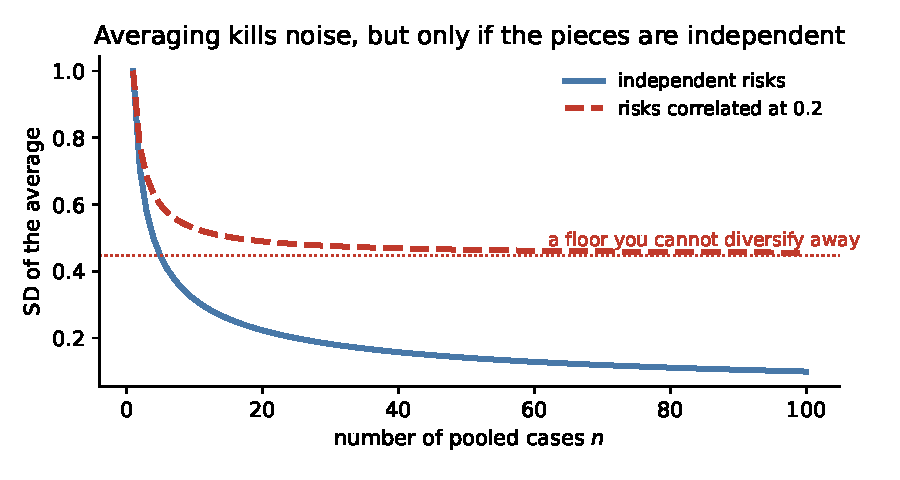
\includegraphics[width=\textwidth]{fig_m06_pooling.pdf}
\end{column}
\begin{column}{0.42\textwidth}
\small
The SD of an average of $n$ independent cases falls like $1/\sqrt{n}$.
\begin{itemize}
  \item Four times the data, half the noise. That is the entire economics of sample size, and you
        met it in Unit 1 as $\sigma/\sqrt{n}$.
  \item If the cases are correlated, the curve flattens onto a floor you cannot buy your way
        below.
\end{itemize}
\end{column}
\end{columns}
\onslide<2->{\centering\small
This one picture is insurance, portfolio diversification, and A/B testing, and also why a pandemic
or a market crash breaks all three at once.}
\end{frame}

\begin{frame}{Your turn \#4}
\begin{yourturn}{same average, different animal}
Two ad campaigns each have an expected return of \$50{,}000.
\begin{itemize}
  \item Campaign A returns somewhere between \$40k and \$60k.
  \item Campaign B has a 90\% chance of \$0 and a 10\% chance of \$500k.
\end{itemize}
With a neighbor: which do you recommend, and what do you need to know about the company first?
\end{yourturn}
\end{frame}

\begin{frame}{Your turn \#4: answer}
\begin{itemize}
  \item There is no answer without context. The real questions are \textbf{how many times you get
        to play} and \textbf{what a zero costs you}.
  \item A firm running 50 campaigns a year should take B. The averaging in the last picture turns
        its variance into a reliable return.
  \item A startup that must make payroll next month should take A. One draw of \$0 ends the
        company, and there is no long run for a company that no longer exists.
\end{itemize}
\begin{principle}{expected value assumes you survive to repeat}
Maximize expected value across many bets you can absorb. For a single bet you cannot recover from,
look at the downside instead.
\end{principle}
\end{frame}

\begin{frame}{Pick the distribution by the mechanism}
\begin{columns}[c]
\begin{column}{0.6\textwidth}
\centering
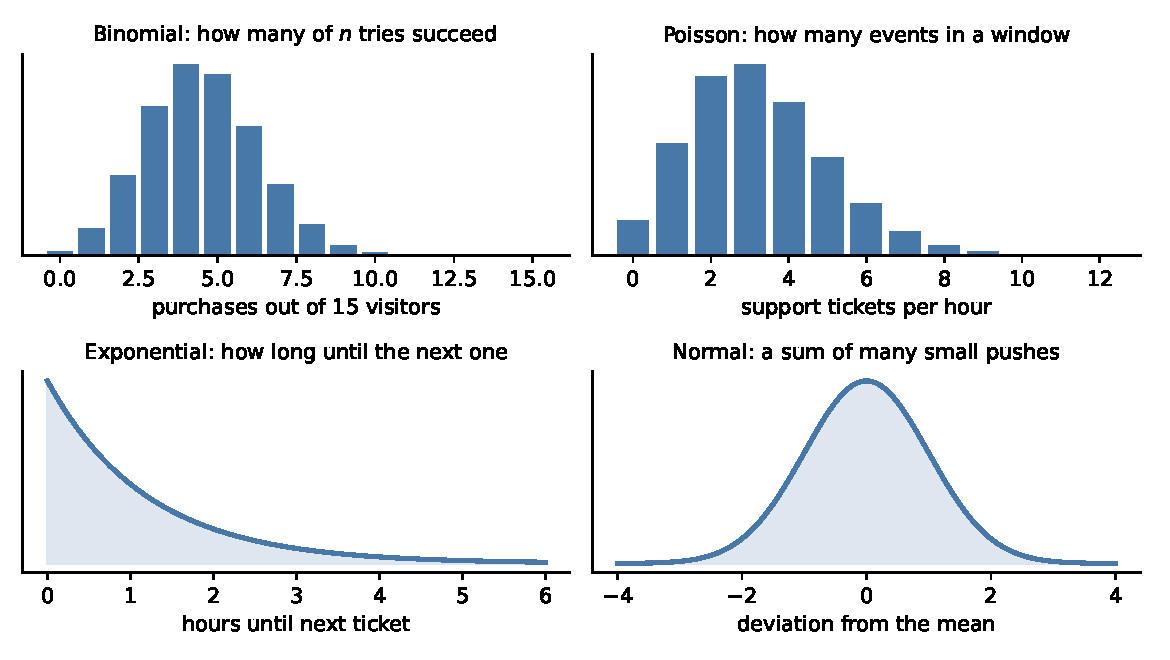
\includegraphics[width=\textwidth]{fig_m06_dists.pdf}
\end{column}
\begin{column}{0.4\textwidth}
\small
Each shape comes from a \emph{story} about how the data is generated. Learn the four stories and
the formulas follow.
\end{column}
\end{columns}
\end{frame}

\begin{frame}{The four stories worth memorizing}
\begin{itemize}
  \item \textbf{Bernoulli / Binomial:} a fixed number of independent yes-or-no tries, each with
        the same chance. ``How many of 500 visitors converted?'' $\E{X} = np$,
        $\Var{X} = np(1-p)$.
  \item \textbf{Poisson:} events arriving at a steady rate in a window of time or space. ``How
        many tickets this hour?'' Mean and variance are both $\lambda$.
  \item \textbf{Exponential:} the waiting time \emph{until} the next such event.
  \item \textbf{Normal:} anything built from many small independent contributions added together.
        Unit 3 is entirely about why this one shows up everywhere.
\end{itemize}
\end{frame}

\begin{frame}{Choosing a model in practice}
\begin{itemize}
  \item Ask what generated the number, not what the histogram looks like.
  \item Counts of successes out of a known number of tries: binomial. Counts with no natural
        ceiling, arriving over time: Poisson.
  \item Waiting times, durations, and time-to-failure: exponential-ish, and almost always
        right-skewed.
  \item Money is almost never normal. Revenue per customer, income, and claim sizes are skewed
        with a long right tail.
\end{itemize}
\begin{trap}{a check worth running}
Poisson forces the variance to equal the mean. Real count data is usually \emph{over}-dispersed,
with variance well above the mean, because the underlying rate itself varies (Mondays, launches,
outages). Check that before trusting a Poisson.
\end{trap}
\end{frame}

\begin{frame}{Averages plugged into nonlinear things}
\begin{columns}[c]
\begin{column}{0.58\textwidth}
\centering
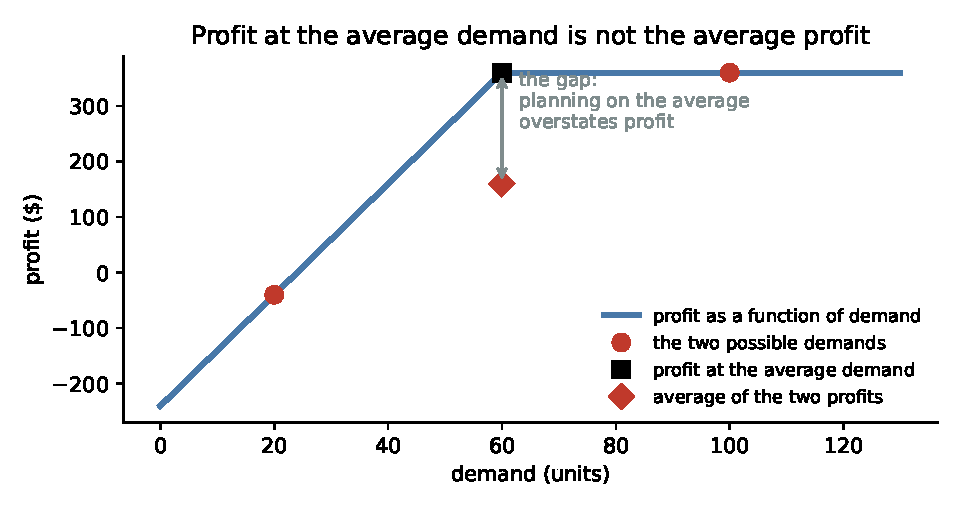
\includegraphics[width=\textwidth]{fig_m06_flaw.pdf}
\end{column}
\begin{column}{0.42\textwidth}
\small
Capacity is 60 units, each sold for \$10, each unit of capacity costs \$4. Demand is 20 or 100,
equally likely.
\begin{itemize}
  \item Profit at the \emph{average} demand of 60: \textbf{\$360}.
  \item \emph{Average} profit across the two demands: \textbf{\$160}.
\end{itemize}
The plan built on the average overstates profit by more than double.
\end{column}
\end{columns}
\end{frame}

\begin{frame}{Why the gap appears}
\begin{itemize}
  \item Whenever the quantity you care about is a \textbf{curved} function of an uncertain input,
        $\E{f(X)} \neq f(\E{X})$.
  \item Caps, floors, thresholds, penalties, stockouts, and SLA cliffs are all curves. Business is
        made of them.
  \item ``A statistician drowned crossing a river of average depth three feet.''
\end{itemize}
\begin{trap}{planning on the average}
Any plan built by replacing every uncertain input with its mean will be systematically wrong, and
usually optimistic, because it ignores the bad tail where the penalties live.
\end{trap}
\end{frame}

\begin{frame}{The mean is not the typical case}
\begin{columns}[c]
\begin{column}{0.58\textwidth}
\centering
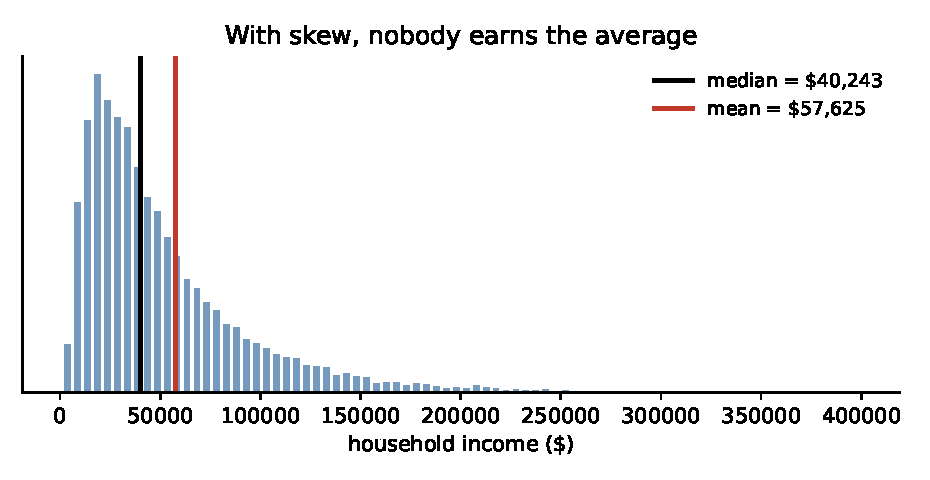
\includegraphics[width=\textwidth]{fig_m06_skew.pdf}
\end{column}
\begin{column}{0.42\textwidth}
\small
With right-skewed data the mean sits well above the median, dragged up by the tail.
\begin{itemize}
  \item ``Average revenue per user'' in a business where 2\% of users are whales describes nobody.
  \item Report the median, the mean, and something about the tail. They answer different
        questions.
\end{itemize}
\end{column}
\end{columns}
\onslide<2->{\centering\small
Rule of thumb: when the mean and median differ a lot, someone is about to be misled.}
\end{frame}

% ======================================================================
\section{LLM check}
% ======================================================================
\begin{frame}{LLM check: mistake or not? (1 of 2)}
\begin{llmcheck}{we asked an LLM about a screening result}
\textbf{We told it:} ``A test is 99\% accurate. The disease affects 1 in 1000 people. I tested
positive. What is the chance I have it?''\\[4pt]
\textbf{It answered:} ``The test is 99\% accurate, so there is about a 99\% chance you have the
disease. You should follow up with your doctor immediately.''
\end{llmcheck}
\vspace{0.2em}
\centering\small Mistake, or no mistake?
\onslide<2->{%
\begin{trap}{verdict: mistake}
It ignored the base rate. In 100,000 people, 100 are sick (99 test positive) and 99,900 are
healthy (about 999 test positive anyway). The real answer is near \textbf{9\%}, not 99\%.
\end{trap}}
\end{frame}

\begin{frame}{LLM check: mistake or not? (2 of 2)}
\begin{llmcheck}{a question about combining risks}
\textbf{We told it:} ``Our two suppliers each fail 3\% of the time. What is the chance both fail in
the same week?''\\[4pt]
\textbf{It answered:} ``If the failures were independent it would be about 0.09\%, but I would not
rely on that. If both ship through the same port or region, a storm or a strike takes out both at
once, and the true joint probability could be many times higher. I would ask what the two
suppliers have in common before quoting a number.''
\end{llmcheck}
\vspace{0.2em}
\centering\small Mistake, or no mistake?
\onslide<2->{%
\begin{principle}{verdict: no mistake}
It gives the independent calculation, labels the assumption, and goes looking for the shared
cause. That is the habit from Day 1, applied correctly.
\end{principle}}
\end{frame}

% ======================================================================
\section{Consolidate}
% ======================================================================
\begin{frame}{How to attack any probability question, in order}
\begin{enumerate}
  \item \textbf{Name the events} precisely, in words, before any arithmetic.
  \item \textbf{Write down which conditional you were given} and which one you were asked for. If
        they differ, you need Bayes.
  \item \textbf{Find the base rate.} If nobody has mentioned one, that is your missing ingredient.
  \item \textbf{Build a table of 10,000 cases} instead of manipulating formulas.
  \item \textbf{Check the independence} of anything you multiplied. What would make these events
        move together?
  \item \textbf{For a quantity, report a mean and a spread}, and simulate rather than plugging in
        averages.
\end{enumerate}
\end{frame}

\begin{frame}{Turning a probability question into arithmetic}
\small
\begin{enumerate}
  \item \textbf{Name the events in words} and write which conditional you were given.
  \item \textbf{Ask which one you were asked for.} If it is the other direction, you need Bayes.
  \item \textbf{Find the base rate.} If nobody stated one, that is your missing input.
  \item \textbf{Build a table of 10{,}000 cases}: prevalence splits the column, sensitivity and specificity split each row.
  \item \textbf{Read the answer off the table} as a ratio of counts, not a formula.
  \item \textbf{Check any multiplication} you did for a shared cause before trusting independence.
  \item \textbf{If it is a quantity rather than an event}, report a mean \emph{and} an SD, and simulate rather than plugging in averages.
\end{enumerate}
\end{frame}

\begin{frame}{The traps, all in one place}
\begin{trap}{the ones that bite most often}
\begin{itemize}
  \item Flipping a conditional: reporting $\PR{B \mid A}$ when the question asked
        $\PR{A \mid B}$.
  \item Ignoring the base rate after a positive test or a model flag.
  \item Multiplying probabilities of events that share a common cause.
  \item Believing chance ``evens out'' in the short run.
  \item Ranking small groups by rates and believing the extremes.
  \item Reporting a mean with no spread, or calling it typical when the data is skewed.
  \item Computing the answer at average inputs instead of averaging the answers.
\end{itemize}
\end{trap}
\end{frame}

\begin{frame}{Ten questions to be able to answer}
\begin{enumerate}\small
  \item A 99\%-accurate test for a 1-in-1000 disease comes back positive. Now what?
  \item Explain the difference between $\PR{A \mid B}$ and $\PR{B \mid A}$ with an example.
  \item What does independence require, and when have you seen it assumed wrongly?
  \item A coin lands heads six times in a row. What is the chance of heads next?
  \item Why is a 1\% daily failure risk a serious problem over a quarter?
  \item Our fraud model flags 2\% of transactions. How would you tell whether it is any good?
  \item Why are the healthiest and the sickest counties both mostly small ones?
  \item Two projects have equal expected return. What else do you want to know?
  \item Why is profit at average demand not the same as average profit?
  \item Your count data has variance three times its mean. What does that tell you?
\end{enumerate}
\end{frame}

\begin{frame}{Mastery checklist}
You have this unit when you can, from memory:
\begin{itemize}
  \item use complement, addition, and multiplication rules without confusing them
  \item say precisely what independence requires, and spot a shared cause
  \item translate any accuracy claim into a conditional probability, in the right direction
  \item solve a Bayes problem by counting 10,000 people
  \item define expectation and standard deviation, and use linearity to break a total into pieces
  \item say what happens to the mean and SD when independent things are summed or averaged
  \item match binomial, Poisson, exponential, and normal to their generating stories
  \item explain the flaw of averages with a concrete example
\end{itemize}
\end{frame}

\begin{frame}{What you should be able to do with software}
\small
Nobody is asking you to memorize syntax. You are expected to know \emph{which} procedure the
question calls for, what to hand it, and what the output means. With an AI assistant open, you
should be able to produce any of these and defend the result.
\begin{center}\footnotesize
\begin{tabular}{p{0.44\textwidth} p{0.46\textwidth}}
\toprule
\textbf{You should be able to} & \textbf{What you would reach for} \\
\midrule
Simulate any event and estimate its probability & \texttt{rng.random}, \texttt{rng.integers} \\
Exact binomial probabilities and tails & \texttt{stats.binom.pmf}, \texttt{.cdf}, \texttt{.sf} \\
Counts over a window (Poisson) & \texttt{stats.poisson.pmf}, \texttt{.sf} \\
Waiting times & \texttt{stats.expon} \\
A natural-frequency screening table & a few lines of arithmetic, no library \\
Mean and SD of a simulated quantity & \texttt{.mean()}, \texttt{.std(ddof=1)} \\
Expected cost or profit under uncertainty & simulate the scenarios, then average \\
\bottomrule
\end{tabular}
\end{center}
\vspace{0.2em}
\centering\small
If you cannot say what the output means, the fact that you produced it is worth nothing.
\end{frame}

\begin{frame}{Where we go next}
\begin{itemize}
  \item We just saw that averages of many independent pieces get predictably tighter, like
        $1/\sqrt{n}$. \textbf{Unit 3} explains why, and shows that they also take on a specific
        \emph{shape}, almost regardless of what you averaged.
  \item That result is what makes the standard error from Unit 1 computable, and it is the
        foundation under every interval in the course.
\end{itemize}
\begin{principle}{the habit to keep}
Report a spread with every number. The mean says where things sit, the SD says how far they
move.
\end{principle}
\end{frame}

\end{document}
